\section{Motivation}
\label{sec:motivation}

\begin{figure}
    \centering
    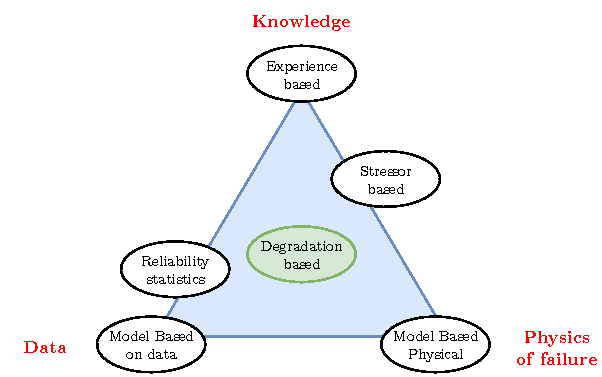
\includegraphics[scale=1.3]{images/Intro/MaintTriangle.pdf}
    \caption{Maintenance triangle}
    \label{fig:MaintTriangle}
\end{figure} 

Takin for example a survey published by the U.S. Department of Commerce in 2020, the maintenance expenditure of the manufacturing industry in the USA was \$57.3 billion, while the losses due to preventable maintenance issues amounted to \$119.1 billion. The top 25\% of those 
establishments relying on reactive maintenance were associated with 3.3 times more downtime 
than those in the bottom 25\% \cite{NIST}. This means that the economic impact of failures exceeds the cost of maintenance by a factor of 2.1, and this is concentrated in those sectors that rely more on reactive maintenance. The aforementioned emphasizes the importance of developing a general purpose \gls{pdm} system that can be applied in a large variety of systems.

In the article \cite{Maintenance_cat}, the authors divide the \gls{cbm} strategies in five categories:

\begin{itemize}
    \item \emph{experience based} predictions are based on the experience and knowledge outside or within the company. It is based on little scattered data on average conditions. The only  requirement is that the experience of the experts is quantified and used;
    \item \emph{reliability statistics} predictions are based on the statistical analysis of the failure data without considering the specific system. These methods also estimate the life
    of an average component operating under historically average conditions;
    \item \emph{stressor based} predictions can be considered an extension of the reliability statistics methods. The difference is that they also consider a measure of the stress (humidity, temperature, etc.) that the component is exposed to;
    \item \emph{degradation based} predictions are based on the extrapolation of the degradation of the component;
    \item \emph{model based} predictions are based on the knowledge of the physics of the system. The assumption is that the degradation can be computed instead of measured. They can be based on a physical model or on a data-driven model.
\end{itemize}


The authors of \cite{Maintenance_cat} also propose a distribution of these categories in a triangle, as shown in \autoref{fig:MaintTriangle}. Each vertex represents a requisite for the implementation, and the distance of the method to the vertex represents how dependent it is on that requisite. To obtain a general purpose \gls{pdm} framework, the \emph{degradation based} approach seems the most promising, since it is the least dependent on a specific requisite.

Moreover, to enhance even more the general purpose nature of the framework, a \gls{uml} model can be chosen. This speeds up the implementation of the framework on a machine about which little is known, plus, it can be implemented on a new machine without a deep knowledge of the \gls{uml} algorithms themself.

In the paper \cite{GridPredictMaintenance}, it is pointed out that \gls{glo:edge} implementations, not only enable the use of the framework for special applications but also enhance the cybersecurity of facilities that may not need an edge implementation due to technical limitations.